%% LyX 2.3.2 created this file.  For more info, see http://www.lyx.org/.
%% Do not edit unless you really know what you are doing.
\documentclass[11pt,a4paper,english]{desearticle}
\usepackage{mathptmx}
\usepackage{helvet}
\usepackage{courier}
\renewcommand{\familydefault}{\rmdefault}
\usepackage[latin9]{inputenc}
\usepackage{fancyhdr}
\pagestyle{fancy}
\usepackage{float}
\usepackage{booktabs}
\usepackage{graphicx}

\makeatletter

%%%%%%%%%%%%%%%%%%%%%%%%%%%%%% LyX specific LaTeX commands.
\pdfpageheight\paperheight
\pdfpagewidth\paperwidth

%% Because html converters don't know tabularnewline
\providecommand{\tabularnewline}{\\}

%%%%%%%%%%%%%%%%%%%%%%%%%%%%%% User specified LaTeX commands.
\Author{Student A, Student B}
\Afil{DESE, IISc}
\Journal{Electronic Systems Packaging}
\Month{Oct-Jan}
\Year{2020}

\makeatother

\usepackage{babel}
\begin{document}
\title{{\huge{}Assignment title}}
\maketitle
\begin{abstract}
The abstract section gives the key take-away of the experiment. Do
not confuse abstract with the conclusion section. The abstract is
a summary of the article indicating the most important point that
is addressed. Abstract provides the motivation, aim and scope of the
experiment. Whereas, the conclusion section provides an authors' insight
on the experiment. It gives the thoughts of the authors on the results,
discrepancy in results with respect to theory, any means for addressing
the discrepancies, any interesting and novel applications that can
be considered as spin-offs from this experiment, so on and so forth.
\end{abstract}

\section{Introduction}

This section provides an introduction to the experiment. Discuss the
need for the experiment and how it will be executed? What will be
learned from this experiment? What are the necessary background literature
that you have referred? In this section you will include citation
to the references like datasheets, papers, articles, notes etc. Build
up you list of references in a .bib file in bibtex format. Load the
bibtex into the ``Bibtex generated bibliography'' template at the
end of this article. The references can then be cited in the text
of the article. I will cite two references here that will automatically
get sorted and listed at the end in the references section. \cite{lp3w}
is an arbitrary book reference and \cite{LM741} is a reference to
the data sheet of LM 741 op-amp.

. 

\section{Tasks}

Every experiment will consist of several tasks starting from task-1
to task-n. Something that is common to every experiment is the circuit
diagram. Draw the circuit diagram and explain its operation. Use a
vector graphics program like inkscape to draw the figures and circuit.
Do not cut and paste figures from any sources or references. Another
nice package that you may use is gEDA (gnu Electronics Design and
Automation). Within this package, there is a software called ``gschem''.
This can be used effectively to draw neat circuits. This is actually
a frontend for ngSpice simulation software and also for ``pcb''
which is used to make printed circuit boards.

\subsection*{Task-1}

The first task is to design the experimental circuit. Choose the op
amp. Download the data sheet and study the various parameters. Write
the design equations as a script file in either OCTAVE or MATLAB environment.
Obtain the values of the components. Find out the input-output relationship
under ideal op-amp consideration and also for practical op-amp consideration.

\subsection*{Task-2}

You may also consolidate the experiment with simulation results too.
You can use NgSpice, LTSpice, PSpice, Simscape, octave, etc. for simulating
the circuits. Present the results in the form of tabulations and plots.
I have shown few examples of introducing figures into the article
for relevant tasks.

\begin{figure}[h]
\begin{centering}
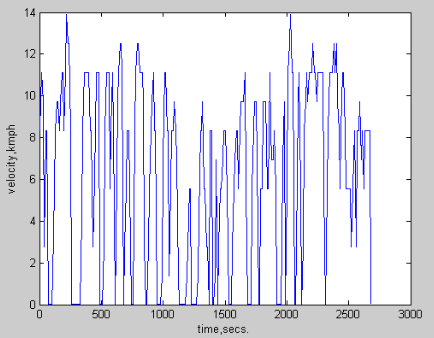
\includegraphics[scale=0.5]{figure1}
\par\end{centering}
\caption{\label{fig:label1}Caption for figure having label as label1}
\end{figure}


\subsection*{Task-3}

Always note that every figure should also be cited in the text. For
example, \ref{fig:label1} if the citation of figure 1. \ref{fig:label2}
is the citation for figure 2 and \ref{tab:table1} cites the tabulation
table 1.

Every figure should have a figure caption. Scale the figure to fit
properly within the column width of the double column format lab report.
Use as many figures as possible to clarify the experiment. Presentation
of results in graphical form alongwith associated textual discussion
is more preferred than only textual discussion.

\begin{figure}[h]
\begin{centering}
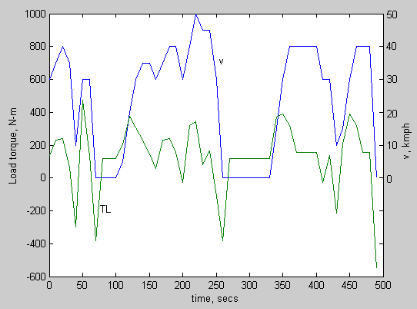
\includegraphics[scale=0.5]{figure2}
\par\end{centering}
\caption{\label{fig:label2}This is caption for figure having label as label2}
\end{figure}


\subsection*{Task-n}

Each experiment may have different number of tasks. Perform all the
tasks. Tabulate the results before plotting. I have indicated an example
of tabulation. Give the tabulation a table number and a table caption.
Kindly also cite the table in the textual discussion.

\begin{table}[H]
\begin{centering}
\begin{tabular}{clll}
\toprule 
\textbf{Sl. No.} & \textbf{param-1} & \textbf{param-2} & \textbf{\%result}\tabularnewline
\midrule
\midrule 
1 & 1e-3 & 0.5 & 0\tabularnewline
\midrule 
2 & 5e-3 & 1.0 & 0.3\tabularnewline
\midrule 
3 & 10e-3 & 1.5 & 0.5\tabularnewline
\midrule 
4 & 20e-3 & 2.0 & 0.3\tabularnewline
\midrule 
5 & 50e-3 & 2.5 & 1.2\tabularnewline
\bottomrule
\end{tabular}
\par\end{centering}
\caption{\label{tab:table1}Caption for table with label as table1}

\end{table}

\begin{figure}[h]
\begin{centering}
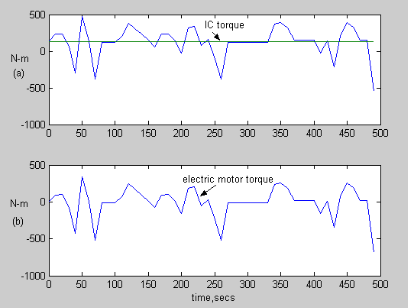
\includegraphics[scale=0.5]{figure3}
\par\end{centering}
\caption{\label{fig:label3}(a) Caption for part-a of figure (b) Caption for
part-b of figure}
\end{figure}


\section{Conclusions}

In most cases, the experimental results will not match theoretical
calculations. This sections addresses this by discussion on these
mismatches. This is a very important section. It provides an insight
into the authors' thought flow. Note that this section is not merely
a summary of the entire article. It discusses the experiment from
the angle of practicalities and uncertainities. As there are no ideal
situations in practical realisations, the authors should discuss on
aspects where the result is not as expected by theory. In what ways
the short comings in the theory can be addressed? What are the possible
solutions? Brainstorming is an essential component of this section.
The authors can also put forth comparisons based on similar circuits,
simulation results and discussions in literature to consolidate the
results that have been obtained in this experiment.

\bibliographystyle{unsrt}
\bibliography{report}

\end{document}
